%---------------------------------------------------------------------------------
% HEADER
%---------------------------------------------------------------------------------
% Stanford - ME227 Spring 2021
% Instructor: Chris Gerdes
% TA's: Peter Schleede, John Talbot
%
% This is a borrowed LaTeX template file for lecture notes for CS267,
% Applications of Parallel Computing, UCBerkeley EECS Department.
%
% PLEASE MODIFY THIS TEMPLATE ONLY WHERE MARKED WITH "STUDENT:"
%
% The only parts that need to be modified in this document
% are found in each of the invididual prompt files which are found in problem folders (e.g. Problem1/problem1a.tex). 
%


\documentclass[10pt]{exam}

%---------------------------------------------------------------------------------
% ADD PACKAGES
%---------------------------------------------------------------------------------
% Built in packages
\usepackage[utf8]{inputenc}
\usepackage{amsmath}
\usepackage[title]{appendix}
\usepackage{empheq}
\usepackage{fmtcount}
\usepackage{graphicx}
\usepackage{hyperref}
\usepackage[numbered,framed]{matlab-prettifier}
\usepackage{mdframed}
\usepackage{minibox}
\usepackage{siunitx}
\usepackage{stackengine}
\usepackage{xcolor}
\usepackage{xpatch}

%Disable all warnings issued by latex starting with "You have..."
\usepackage{silence}
\WarningFilter{latex}{You have requested package}

% Custom packages
\usepackage{Utility/undertilde}

% Custom functions and macros

% This is a borrowed LaTeX template file for lecture notes for CS267,
% Applications of Parallel Computing, UCBerkeley EECS Department.
% Now being used for CMU's 10725 Fall 2012 Optimization course
% taught by Geoff Gordon and Ryan Tibshirani.  When preparing 
% LaTeX notes for this class, please use this template.
%
% To familiarize yourself with this template, the body contains
% some examples of its use.  Look them over.  Then you can
% run LaTeX on this file.  After you have LaTeXed this file then
% you can look over the result either by printing it out with
% dvips or using xdvi. "pdflatex template.tex" should also work.

\setlength{\oddsidemargin}{0 in}
\setlength{\evensidemargin}{0 in}
\setlength{\topmargin}{-0.6 in}
\setlength{\textwidth}{6.5 in}
\setlength{\textheight}{8.5 in}
\setlength{\headsep}{0.75 in}
\setlength{\parindent}{0 in}
\setlength{\parskip}{0.1 in}
\extrafootheight{-0.5in}

% flags to display template, solution, or condensed versions
% toggletrue{variable} or togglefalse{variable}
% nothing stopping you from turning all 3 on and getting a 
% super long document
\newtoggle{template}
\newtoggle{solution}
\newtoggle{condensed}
\newtoggle{student}

\newcommand{\template}{
    \toggletrue{template}
    \togglefalse{solution}
    \togglefalse{condensed}
    \togglefalse{student}
}

\newcommand{\solutions}{
    \toggletrue{solution}
    \togglefalse{template}
    \togglefalse{condensed}
    \togglefalse{student}
}

\newcommand{\condensed}{
    \toggletrue{condensed}
    \togglefalse{template}
    \togglefalse{solution}
    \togglefalse{student}
}

\newcommand{\student}{
    \toggletrue{student}
    \togglefalse{template}
    \togglefalse{solution}
    \togglefalse{condensed}
}

%% For hw6
%\newcommand*\circled[1]{\tikz[baseline=(char.base)]{
%    \node[shape=circle,draw,inner sep=2pt] (char) {#1};}}
%
%% The following commands set up the lecnum (lecture number)
%% counter and make various numbering schemes work relative
%% to the lecture number.

\newcounter{lecnum}

%\renewcommand{\thepage}{\thelecnum.\arabic{page}}
%\renewcommand{\thesection}{\thelecnum.\arabic{section}}
\renewcommand{\thesubsection}{\arabic{section}.\Alph{subsection}}
\renewcommand{\theequation}{\thelecnum.\arabic{equation}}
\renewcommand{\thefigure}{\thelecnum.\arabic{figure}}
\renewcommand{\thetable}{\thelecnum.\arabic{table}}

%\newcommand{\cc}{{\circ}}
%\newcommand{\Cf}{{\tilde{C}_{f\cc}}}
%\newcommand{\Cr}{{\tilde{C}_{r\cc}}}
%\newcommand{\Kpf}{{K_{\phi f}}}
%\newcommand{\Kpr}{{K_{\phi r}}}
%\newcommand{\Kp}{{K_{\phi}}}
%\newcommand{\cs}{{c_\mathrm{sky}}}


%
% The following macro is used to generate the header.
%
\newcommand{\lecture}[4]{
   \pagestyle{myheadings}
   \thispagestyle{plain}
   \newpage
   \setcounter{lecnum}{#1}
   \setcounter{page}{1}
   \noindent
   \begin{center}
   \framebox{
      \vbox{\vspace{2mm}
    \hbox to 6.28in { {\bf ME227: Vehicle Dynamics and Control
	\hfill Spring 2021} }
       \vspace{4mm}
       \hbox to 6.28in { {\Large \hfill Lecture #1: #2  \hfill} }
       \vspace{2mm}
       \hbox to 6.28in { {#3 \hfill \textcopyright #4 } }
      \vspace{2mm}}
   }
   \end{center}
   \markboth{Lecture #1: #2}{Lecture #1: #2}

}

\newcommand{\assignment}[4]{
   \pagestyle{myheadings}
   \thispagestyle{plain}
   \newpage
   \setcounter{lecnum}{#1}
   \setcounter{page}{1}
   \noindent
   \begin{center}
   \framebox{
      \vbox{\vspace{2mm}
    \hbox to 6.28in { {\bf ME227: Vehicle Dynamics and Control
	\hfill Spring 2021} }
       \vspace{4mm}
       \hbox to 6.28in { {\Large \hfill Assignment #1: #2  \hfill} }
       \vspace{2mm}
       \hbox to 6.28in { {#3 \hfill \textcopyright #4 } }
      \vspace{2mm}}
   }
   \end{center}
   \markboth{Assignment #1: #2}{Assignment #1: #2}
}

\newcommand{\solutionME}[4]{
   \pagestyle{myheadings}
   \thispagestyle{plain}
   \newpage
   \setcounter{lecnum}{#1}
   \setcounter{page}{1}
   \noindent
   \begin{center}
   \framebox{
      \vbox{\vspace{2mm}
    \hbox to 6.28in { {\bf ME227: Vehicle Dynamics and Control
	\hfill Spring 2017} }
       \vspace{4mm}
       \hbox to 6.28in { {\Large \hfill Solution #1: #2  \hfill} }
       \vspace{2mm}
       \hbox to 6.28in { {#3 \hfill \textcopyright #4 } }
      \vspace{2mm}}
   }
   \end{center}
   \markboth{Solution #1: #2}{Solution #1: #2}
}

\newcommand{\project}[4]{
   \pagestyle{myheadings}
   \thispagestyle{plain}
   \newpage
   \setcounter{lecnum}{#1}
   \setcounter{page}{1}
   \noindent
   \begin{center}
   \framebox{
      \vbox{\vspace{2mm}
    \hbox to 6.28in { {\bf ME227: Vehicle Dynamics and Control
	\hfill Spring 2020} }
       \vspace{4mm}
       \hbox to 6.28in { {\Large \hfill Project: #2  \hfill} }
       \vspace{2mm}
       \hbox to 6.28in { {#3 \hfill \textcopyright #4 } }
      \vspace{2mm}}
   }
   \end{center}
   \markboth{Project: #2}{Project: #2}
}

%
% Convention for citations is authors' initials followed by the year.
% For example, to cite a paper by Leighton and Maggs you would type
% \cite{LM89}, and to cite a paper by Strassen you would type \cite{S69}.
% (To avoid bibliography problems, for now we redefine the \cite command.)
% Also commands that create a suitable format for the reference list.
\renewcommand{\cite}[1]{[#1]}
\def\beginrefs{\begin{list}%
        {[\arabic{equation}]}{\usecounter{equation}
         \setlength{\leftmargin}{2.0truecm}\setlength{\labelsep}{0.4truecm}%
         \setlength{\labelwidth}{1.6truecm}}}
\def\endrefs{\end{list}}
\def\bibentry#1{\item[\hbox{[#1]}]}

%Use this command for a figure; it puts a figure in wherever you want it.
%usage: \fig{NUMBER}{SPACE-IN-INCHES}{CAPTION}

% Use these for theorems, lemmas, proofs, etc.
\newtheorem{theorem}{Theorem}[lecnum]
\newtheorem{lemma}[theorem]{Lemma}
\newtheorem{proposition}[theorem]{Proposition}
\newtheorem{claim}[theorem]{Claim}
\newtheorem{corollary}[theorem]{Corollary}
\newtheorem{definition}[theorem]{Definition}
\newenvironment{proof}{{\bf Proof:}}{\hfill\rule{2mm}{2mm}}

% **** IF YOU WANT TO DEFINE ADDITIONAL MACROS FOR YOURSELF, PUT THEM HERE:

\newcommand\E{\mathbb{E}}

\newcommand{\eX}{{\boldsymbol{\hat{e}_X}}}
\newcommand{\eY}{{\boldsymbol{\hat{e}_Y}}}
\newcommand{\eZ}{{\boldsymbol{\hat{e}_Z}}}
\newcommand{\pVE}{{\psi_{VE}}}
\newcommand{\pVEdot}{\dot{\psi}_{VE}}

%\newcommand{\roa}{\uvec{r}_{oa}}

% basis vector: arg1 is name
\newcommand{\basvec}[1]{\boldsymbol{\hat{e}_{#1}}}

% "radius" vector (position vector named r) from arg1 to arg2

\renewcommand{\vec}[1]{%
  \smash{\ensurestackMath{\stackengine{1pt}{#1}{\scriptscriptstyle\sim}{U}{c}{F}{F}{S}}}
  \vphantom{#1}
}
\newcommand{\roa}{\vec{r}_{oa}}
\newcommand{\rv}[3]{\vec{r}_{#1#2,#3}}


% similar with velocity and acceleration vectors
\newcommand{\vv}[3]{\vec{v}_{#1#2,#3}}
\newcommand{\wv}[3]{\vec{\omega}_{#1#2,#3}}
\newcommand{\av}[3]{\vec{a}_{#1#2,#3}}

% vector derivatives
\newcommand{\drv}[3]{\vec{\dot{r}}_{#1#2,#3}}
\newcommand{\dvv}[3]{\vec{\dot{v}}_{#1#2,#3}}
\newcommand{\dwv}[3]{\vec{\dot{\omega}}_{#1#2,#3}}

% forces
\newcommand{\F}[2]{\text{F}_\text{#1#2}}

% cornering stiffnesses and slip angles
\newcommand{\Caf}{C_{\alpha f}}
\newcommand{\Car}{C_{\alpha r}}
\newcommand{\af}{\alpha f}
\newcommand{\ar}{\alpha r}

% vehicle states and derivatives
\newcommand{\Uxdot}{\dot{U}_x}
\newcommand{\Uydot}{\dot{U}_y}
\newcommand{\rdot}{\dot{r}}
\newcommand{\dpsi}{\Delta\Psi}
\newcommand{\dpsidot}{\Delta\dot{\Psi}}
\newcommand{\edot}{\dot{e}}

% Gains
\newcommand{\Kla}{K_{la}}
\newcommand{\xla}{x_{la}}

% Commands for Gradescope and Grader
\newcommand{\GS}{\textbf{Gradescope}}
\newcommand{\GR}{\textbf{MATLAB Grader}}
\newcommand{\MO}{\textbf{MATLAB Online}}
\newcommand{\GSno}{Gradescope}
\newcommand{\GRno}{MATLAB Grader}
\newcommand{\MOno}{MATLAB Online}
\newcommand{\M}{MATLAB}
% Commands for numberless section headings while incrementing counter
\newcommand{\secNoNum}[1]{\refstepcounter{section}\section*{#1}}
\newcommand{\subsecNoNum}[1]{\refstepcounter{subsection}\subsection*{#1}}
\newcommand{\ph}{Problem \thesection}
\newcommand{\qh}{Question \thesection.\Alph{subsection}}
\newcommand{\apph}{Appendix \Alph{section}}

% Commands for questions subsection headings
\newcommand{\secPr}[1]{%
    \secNoNum{%
        \ph{} -- #1
    }
    \label{sec:#1}
}

\newcommand{\secApp}[1]{%
    \secNoNum{%
        \apph{} -- #1
    }
    \label{appendix:#1}
}

\newcommand{\secGR}[1]{%
    \subsecNoNum{%
        \color{blue}
        \qh{} -- #1 (\GRno{})
    }
    \label{subsecGR:#1}
}

\newcommand{\secMOGR}[1]{%
    \subsecNoNum{%
        \color{blue}
        \qh{} -- #1 (\MOno{} / \GRno{})
    }
    \label{subsecMOGR:#1}
}

\newcommand{\secMOGS}[1]{%
    \subsecNoNum{%
        \qh{} -- #1 (\MOno{} / \GSno{})
    }
    \label{subsecMOGS:#1}
}

\newcommand{\secGS}[1]{%
    \subsecNoNum{%
        \qh{} -- #1 (\GSno{})
    }
    \label{subsecGS:#1}
}

% Reference other question subsections
\newcommand{\qrefGR}[1]{%
    \textbf{%
        Question \ref{subsecGR:#1}%
    }%
}

\newcommand{\qrefGS}[1]{%
    \textbf{%
        Question \ref{subsecGS:#1}%
    }%
}

\newcommand{\qrefMOGR}[1]{%
    \textbf{%
        Question \ref{subsecMOGR:#1}%
    }%
}

\newcommand{\qrefMOGS}[1]{%
    \textbf{%
        Question \ref{subsecMOGS:#1}%
    }%
}

\newcommand{\pref}[1]{%
    \textbf{%
        Problem \ref{sec:#1}%
    }%
}


% Shortcut for equation
\newcommand{\eq}[1]{%
    \begin{equation*}
        #1
    \end{equation*}
}

% Shortcut for align
\newcommand{\al}[1]{%
    \begin{align*}
        #1
    \end{align*}
}

% Shortcut for problem expectation
\newcommand{\expect}[1]{%
    \textbf{%
        \textit{%
            #1%
        }%
    }%
}

% Shortcut for bold
\newcommand{\bld}[1]{\textbf{#1}}

% Change solution title
\renewcommand{\solutiontitle}{\noindent\enspace}

% Matlab code helper macros
\newcommand{\matin}[1]{\lstinline[style=Matlab-editor]{#1}}
\newcommand{\matld}[1]{\lstinputlisting[style=Matlab-editor, basicstyle=\footnotesize]{#1}}

% Remove question numbers
\qformat{}
\renewcommand{\questionshook}{%
\setlength{\leftmargin}{0pt}%
\setlength{\labelwidth}{-\labelsep}%
}

% Fix duplicate question labeling
\makeatletter
\xpatchcmd{\questions}
  {question@\arabic{question}}
  {question@\arabic{page}@\arabic{question}}
  {}{}
\makeatother

% Shortcut for underline and bold
\newcommand{\ubf}[1]{\underline{\textbf{#1}}}



% Select mode (select only one at a time)
%\template
\condensed
%\solutions
%\student

%---------------------------------------------------------------------------------
% BEGIN DOCUMENT & INTRO
%---------------------------------------------------------------------------------
\begin{document}
\assignment{6}{Linearization and Project Reflection}{Due Thursday, May 27 at 5:00pm PST}{Chris Gerdes, 2017}

\hspace{0.5cm}

\section*{Purpose}

For this homework, we will study linearization, reflect on the project, and start thinking about racing.

\section*{Instructions}

This homework assignment will be submitted using \GSno{}.

All written portions must be turned in through Gradescope. See the Piazza post on homework guidelines for more
instructions on the different homework resources available to you. Whatever format you decide to use, please \fbox{\textbf{BOX}} all of your final answers.



\newpage

\input{Body/MFTire.tex}


%---------------------------------------------------------------------------------
% PROBLEM 1
%---------------------------------------------------------------------------------
% Problem Intro
\secPr{Weight Distribution and Cornering Stiffness}

Both tire corning stiffness and weight distribution play a role in determining the car’s understeer gradient.  While some properties depend only upon the understeer gradient, other properties of the response depend upon the specific combination of weight balance and cornering stiffnesses that produced that understeer gradient.  Let’s look at how cars with the same understeer gradient can vary in transient performance. 

\iftoggle{condensed}{}{
    \vspace*{1cm}
}


% Student Prompts and Responses
%---------------------------------------------------------------------------------
% QUESTION 1.A
%---------------------------------------------------------------------------------
\secGR{Determining an Appropriate Lookahead Gain}

Let's start with the "lookdown" controller ($x_{la} = 0$). Our first step is to determine a gain that seems physically
reasonable.

Follow the prompts in \GRno{} to create a script to calculate $K_{la}$ such that our controller produces a steer 
angle of 3 degrees when the lateral error is one meter and the vehicle is pointed straight along the path.

You are to modify the lookahead gain, \verb!K_la!, to the appropriate value.

\vspace*{0.5cm}

\iftoggle{solution}{
    \input{Solutions/matlabgrader.tex}
}



\newpage


%---------------------------------------------------------------------------------
% PROBLEM 2
%---------------------------------------------------------------------------------
% Problem Intro
\secPr{Simulating Vehicles with Different Responses}

In this problem, you will implement a simulation to compare the two cars we have looked at in response to a step steering input. Step inputs are common ways to characterize dynamic systems (both open and closed loop).

\iftoggle{condensed}{}{
    \vspace*{0.5cm}
}

% Student Prompts and Responses
%---------------------------------------------------------------------------------
% PROBLEM 2 - PART A
%---------------------------------------------------------------------------------
\secGR{Simulation}
One way to think about the handling characteristics of a car is that a better handling car more closely tracks the driver’s steering input.  Follow the prompt in \GRno{} to simulate the response of both of these vehicles to a steep steer of 1 degree at 65mph using the simulation you developed last week with the linear tire model and small angle approximations for 4 seconds and plot the yaw rate. 

\iftoggle{condensed}{}{
    \vspace*{0.5cm}
}

\iftoggle{solution}{
    %---------------------------------------------------------------------------------
% PROBLEM 2 - PART A
%---------------------------------------------------------------------------------
\secGR{Simulation}
One way to think about the handling characteristics of a car is that a better handling car more closely tracks the driver’s steering input.  Follow the prompt in \GRno{} to simulate the response of both of these vehicles to a steep steer of 1 degree at 65mph using the simulation you developed last week with the linear tire model and small angle approximations for 4 seconds and plot the yaw rate. 

\iftoggle{condensed}{}{
    \vspace*{0.5cm}
}

\iftoggle{solution}{
    %---------------------------------------------------------------------------------
% PROBLEM 2 - PART A
%---------------------------------------------------------------------------------
\secGR{Simulation}
One way to think about the handling characteristics of a car is that a better handling car more closely tracks the driver’s steering input.  Follow the prompt in \GRno{} to simulate the response of both of these vehicles to a steep steer of 1 degree at 65mph using the simulation you developed last week with the linear tire model and small angle approximations for 4 seconds and plot the yaw rate. 

\iftoggle{condensed}{}{
    \vspace*{0.5cm}
}

\iftoggle{solution}{
    \input{Solutions/Problem2/problem2a.tex}
}

\iftoggle{condensed}{}{
    \newpage
}

}

\iftoggle{condensed}{}{
    \newpage
}

}

\iftoggle{condensed}{}{
    \newpage
}

%---------------------------------------------------------------------------------
% QUESTION 2.B
%---------------------------------------------------------------------------------
\secGS{Reflection of Group Controller}

Now let's move on to your group's controller. Let's take a look at your code once more to make sure that everything was actually implemented correctly. 
Let's again consider whether you think the amount of feedback and feedforward was appropriate in this case.

\textbf{(1) Was everything implemented correctly? If not, what implementation challenges did your team run into?}

\textbf{(2) Did each of your controllers effectively use feedback and feedforward? Support your conclusion with plots of your performance.}


\iftoggle{condensed}{
    \vspace*{0.5cm}
}{
    \subsubsection*{Solution:}
}

\iftoggle{solution}{
    %%---------------------------------------------------------------------------------
% QUESTION 1.A
%---------------------------------------------------------------------------------
\secGR{Determining an Appropriate Lookahead Gain}

Let's start with the "lookdown" controller ($x_{la} = 0$). Our first step is to determine a gain that seems physically
reasonable.

Follow the prompts in \GRno{} to create a script to calculate $K_{la}$ such that our controller produces a steer 
angle of 3 degrees when the lateral error is one meter and the vehicle is pointed straight along the path.

You are to modify the lookahead gain, \verb!K_la!, to the appropriate value.

\vspace*{0.5cm}

\iftoggle{solution}{
    \input{Solutions/matlabgrader.tex}
}


}

\iftoggle{template}{
    \begin{solutionorbox}[5in]
    \end{solutionorbox}
    
    \newpage
}

\iftoggle{student}{
%---------------------------------------------------------------------------------
% STUDENT: BEGIN WORK
%---------------------------------------------------------------------------------
% Please box final answer

%---------------------------------------------------------------------------------
% STUDENT: END WORK
%---------------------------------------------------------------------------------
\newpage
}
%---------------------------------------------------------------------------------
% QUESTION 2.C
%---------------------------------------------------------------------------------
\secGS{Simulating from Equilibrium}

For this problem we will use the simple coupled tire model where $F_x$ is assumed to be known. Incorporate this into your simulation (We will supply verification code). Run your simulation of the three-state bicycle model for 4 seconds using $\delta$ = -10° and $F_{xr}$ equal to the value you computed in Problem 2B. Use the drift equilibrium found in Problem 1D as the initial condition. Plot $U_y$, $r$, and $U_x$ on the same plot. Does Marty hold the drift? What happens? Did you expect this? If you'd like, visualize using \texttt{animateDrift.m}.

\vspace*{0.5cm}


\expect{Include your plot and an explanation of what you see.}


\iftoggle{condensed}{
    \vspace*{0.5cm}
}{
    \subsubsection*{Solution:}
}

\iftoggle{solution}{
    %---------------------------------------------------------------------------------
% QUESTION 2.C
%---------------------------------------------------------------------------------
\secGS{Simulating from Equilibrium}

For this problem we will use the simple coupled tire model where $F_x$ is assumed to be known. Incorporate this into your simulation (We will supply verification code). Run your simulation of the three-state bicycle model for 4 seconds using $\delta$ = -10° and $F_{xr}$ equal to the value you computed in Problem 2B. Use the drift equilibrium found in Problem 1D as the initial condition. Plot $U_y$, $r$, and $U_x$ on the same plot. Does Marty hold the drift? What happens? Did you expect this? If you'd like, visualize using \texttt{animateDrift.m}.

\vspace*{0.5cm}


\expect{Include your plot and an explanation of what you see.}


\iftoggle{condensed}{
    \vspace*{0.5cm}
}{
    \subsubsection*{Solution:}
}

\iftoggle{solution}{
    %---------------------------------------------------------------------------------
% QUESTION 2.C
%---------------------------------------------------------------------------------
\secGS{Simulating from Equilibrium}

For this problem we will use the simple coupled tire model where $F_x$ is assumed to be known. Incorporate this into your simulation (We will supply verification code). Run your simulation of the three-state bicycle model for 4 seconds using $\delta$ = -10° and $F_{xr}$ equal to the value you computed in Problem 2B. Use the drift equilibrium found in Problem 1D as the initial condition. Plot $U_y$, $r$, and $U_x$ on the same plot. Does Marty hold the drift? What happens? Did you expect this? If you'd like, visualize using \texttt{animateDrift.m}.

\vspace*{0.5cm}


\expect{Include your plot and an explanation of what you see.}


\iftoggle{condensed}{
    \vspace*{0.5cm}
}{
    \subsubsection*{Solution:}
}

\iftoggle{solution}{
    \input{Solutions/Problem2/problem2c.tex}
}

\iftoggle{template}{
    \begin{solutionorbox}[6in]
    \end{solutionorbox}
    
    \newpage
}

\iftoggle{student}{
%---------------------------------------------------------------------------------
% STUDENT: BEGIN WORK
%---------------------------------------------------------------------------------
% Please box final answer

%---------------------------------------------------------------------------------
% STUDENT: END WORK
%---------------------------------------------------------------------------------
\newpage
}


}

\iftoggle{template}{
    \begin{solutionorbox}[6in]
    \end{solutionorbox}
    
    \newpage
}

\iftoggle{student}{
%---------------------------------------------------------------------------------
% STUDENT: BEGIN WORK
%---------------------------------------------------------------------------------
% Please box final answer

%---------------------------------------------------------------------------------
% STUDENT: END WORK
%---------------------------------------------------------------------------------
\newpage
}


}

\iftoggle{template}{
    \begin{solutionorbox}[6in]
    \end{solutionorbox}
    
    \newpage
}

\iftoggle{student}{
%---------------------------------------------------------------------------------
% STUDENT: BEGIN WORK
%---------------------------------------------------------------------------------
% Please box final answer

%---------------------------------------------------------------------------------
% STUDENT: END WORK
%---------------------------------------------------------------------------------
\newpage
}



\newpage

%---------------------------------------------------------------------------------
% PROBLEM 3
%---------------------------------------------------------------------------------
% Problem Intro
\secPr{Evaluating our Models Against Experimental Data}

Before plunging deeper into the development of vehicle dynamics models, we should see how well these simple models
predict the measurements we can obtain from a vehicle. We have some data of Niki doing a double lane change maneuver in
the lot off Searsville road on Stanford's campus at various speeds. A high-precision GPS/INS system in the car gives us
accurate measurements of lateral velocity, yaw rate, lateral acceleration, and vehicle speed. We also measure steer
angle through the actuators built into the car. In this problem, we're going to compare these measurements to what we
predict using the models developed in class. While there are a lot of simplifications involved, you should find the
results at least somewhat impressive. If not, chances are you have a bug somewhere...

Three experiments were run, one at low speed, one at intermediate speed, and one at high speed. We have separated all of
the data into MATLAB cell arrays, with the first cell corresponding to the low speed test, etc. 

The following \GRno{} questions will walk you through modifying your simulations so that they can use recorded steer
angle and longitudinal velocity as inputs. With this modification made, you can now compare the experimental data to
three different models.

\textit{NOTE: Though we have written our simulator to execute at 1kHz, our data logger records data on Niki at 200Hz.  In research and industry, we frequently need to resample data that has been logged. One way to address this here is to post-process our recorded data early in our script by creating two new vectors of steering angle and velocity that correspond in time to our simulation time vector. 
You can use the MATLAB function} \verb!interp1! \textit{along with the vector of simulation time to interpolate a vector of
steering angles and velocity from the recorded data. We have implemented this for you in \GRno{}, but it's a great trick to know if
you work with experimental data in the future.}

\vspace*{1cm}


% Student Prompts and Responses
%---------------------------------------------------------------------------------
% QUESTION 3.A
%---------------------------------------------------------------------------------
\secMOGS{Benchmarking Our Setup}

Begin with a brake distribution of 64\%/36\% between the front and rear axle, and roll stiffness Combination A (from Table
\ref{Table:RollParams}). If we want to be able to follow the path within 2m of the desired path, how are we doing at
this point? Which tire saturates at the start of the turn? Is this limit understeer or limit oversteer behavior?  What evidence do we have that this is the case?

\expect{Run the simulation and answer the questions about the vehicle's behavior. Include the tire force plots.}

\iftoggle{condensed}{
    \vspace*{0.5cm}
}{
    \subsubsection*{Solution:}
}

\iftoggle{solution}{
    %---------------------------------------------------------------------------------
% QUESTION 3.A
%---------------------------------------------------------------------------------
\secMOGS{Benchmarking Our Setup}

Begin with a brake distribution of 64\%/36\% between the front and rear axle, and roll stiffness Combination A (from Table
\ref{Table:RollParams}). If we want to be able to follow the path within 2m of the desired path, how are we doing at
this point? Which tire saturates at the start of the turn? Is this limit understeer or limit oversteer behavior?  What evidence do we have that this is the case?

\expect{Run the simulation and answer the questions about the vehicle's behavior. Include the tire force plots.}

\iftoggle{condensed}{
    \vspace*{0.5cm}
}{
    \subsubsection*{Solution:}
}

\iftoggle{solution}{
    %---------------------------------------------------------------------------------
% QUESTION 3.A
%---------------------------------------------------------------------------------
\secMOGS{Benchmarking Our Setup}

Begin with a brake distribution of 64\%/36\% between the front and rear axle, and roll stiffness Combination A (from Table
\ref{Table:RollParams}). If we want to be able to follow the path within 2m of the desired path, how are we doing at
this point? Which tire saturates at the start of the turn? Is this limit understeer or limit oversteer behavior?  What evidence do we have that this is the case?

\expect{Run the simulation and answer the questions about the vehicle's behavior. Include the tire force plots.}

\iftoggle{condensed}{
    \vspace*{0.5cm}
}{
    \subsubsection*{Solution:}
}

\iftoggle{solution}{
    \input{Solutions/Problem3/problem3a.tex}
    \newpage
}

\iftoggle{template}{
    \begin{solutionorbox}[3.5in]
    \end{solutionorbox}
    \newpage
}

\iftoggle{student}{
%---------------------------------------------------------------------------------
% STUDENT: BEGIN WORK
%---------------------------------------------------------------------------------


% Please box final answer

%---------------------------------------------------------------------------------
% STUDENT: END WORK
%---------------------------------------------------------------------------------
    \newpage
}


    \newpage
}

\iftoggle{template}{
    \begin{solutionorbox}[3.5in]
    \end{solutionorbox}
    \newpage
}

\iftoggle{student}{
%---------------------------------------------------------------------------------
% STUDENT: BEGIN WORK
%---------------------------------------------------------------------------------


% Please box final answer

%---------------------------------------------------------------------------------
% STUDENT: END WORK
%---------------------------------------------------------------------------------
    \newpage
}


    \newpage
}

\iftoggle{template}{
    \begin{solutionorbox}[3.5in]
    \end{solutionorbox}
    \newpage
}

\iftoggle{student}{
%---------------------------------------------------------------------------------
% STUDENT: BEGIN WORK
%---------------------------------------------------------------------------------


% Please box final answer

%---------------------------------------------------------------------------------
% STUDENT: END WORK
%---------------------------------------------------------------------------------
    \newpage
}


%---------------------------------------------------------------------------------
% QUESTION 3.B
%---------------------------------------------------------------------------------
\secMOGS{Tuning Roll Stiffness}

Let's try to address our handling problems by adjusting roll stiffness. Combination A has the majority of the stiffness
on the rear axle which is not common for passenger vehicles. Let's try the simulation again with Combination B to see if
we do any better. 

Did this correct the problem we saw with Combination A? Did it create another issue, and if so, what was it? Did we make better progress through
the corner (in other words, is our final distance along the path greater at the end of our 14 second simulation time)?

\vspace*{0.5cm}

\expect{Run the simulation and answer the questions about the vehicle's behavior. Include the tire force plots.}

\iftoggle{condensed}{}{
    \subsubsection*{Solution:}
}

\iftoggle{solution}{
    %---------------------------------------------------------------------------------
% QUESTION 3.B
%---------------------------------------------------------------------------------
\secMOGS{Tuning Roll Stiffness}

Let's try to address our handling problems by adjusting roll stiffness. Combination A has the majority of the stiffness
on the rear axle which is not common for passenger vehicles. Let's try the simulation again with Combination B to see if
we do any better. 

Did this correct the problem we saw with Combination A? Did it create another issue, and if so, what was it? Did we make better progress through
the corner (in other words, is our final distance along the path greater at the end of our 14 second simulation time)?

\vspace*{0.5cm}

\expect{Run the simulation and answer the questions about the vehicle's behavior. Include the tire force plots.}

\iftoggle{condensed}{}{
    \subsubsection*{Solution:}
}

\iftoggle{solution}{
    %---------------------------------------------------------------------------------
% QUESTION 3.B
%---------------------------------------------------------------------------------
\secMOGS{Tuning Roll Stiffness}

Let's try to address our handling problems by adjusting roll stiffness. Combination A has the majority of the stiffness
on the rear axle which is not common for passenger vehicles. Let's try the simulation again with Combination B to see if
we do any better. 

Did this correct the problem we saw with Combination A? Did it create another issue, and if so, what was it? Did we make better progress through
the corner (in other words, is our final distance along the path greater at the end of our 14 second simulation time)?

\vspace*{0.5cm}

\expect{Run the simulation and answer the questions about the vehicle's behavior. Include the tire force plots.}

\iftoggle{condensed}{}{
    \subsubsection*{Solution:}
}

\iftoggle{solution}{
    \input{Solutions/Problem3/problem3b.tex}
}

\iftoggle{template}{
    \begin{solutionorbox}[3.5in]
    \end{solutionorbox}
}

\iftoggle{student}{
%---------------------------------------------------------------------------------
% STUDENT: BEGIN WORK
%---------------------------------------------------------------------------------


% Please box final answer

%---------------------------------------------------------------------------------
% STUDENT: END WORK
%---------------------------------------------------------------------------------
}

\newpage

}

\iftoggle{template}{
    \begin{solutionorbox}[3.5in]
    \end{solutionorbox}
}

\iftoggle{student}{
%---------------------------------------------------------------------------------
% STUDENT: BEGIN WORK
%---------------------------------------------------------------------------------


% Please box final answer

%---------------------------------------------------------------------------------
% STUDENT: END WORK
%---------------------------------------------------------------------------------
}

\newpage

}

\iftoggle{template}{
    \begin{solutionorbox}[3.5in]
    \end{solutionorbox}
}

\iftoggle{student}{
%---------------------------------------------------------------------------------
% STUDENT: BEGIN WORK
%---------------------------------------------------------------------------------


% Please box final answer

%---------------------------------------------------------------------------------
% STUDENT: END WORK
%---------------------------------------------------------------------------------
}

\newpage

%---------------------------------------------------------------------------------
% PROBLEM 3 - PART C
%---------------------------------------------------------------------------------
\secGS{Lookahead vs PD Control}
Show that for a constant vehicle speed, the lookahead controller is equivalent to a PD controller of the form:

\al{
\delta = K_p e + K_d \frac{de}{dt}
}

Calculate the parameters $K_p$ and $K_d$ in terms of $K_{la}$ and $d_{la}$. You should see that the lookahead control law provides a simple way of scaling, or gain scheduling, proportional and derivative gains as the vehicle speed changes.

\vspace*{0.5cm}

\expect{Write the parameters $K_{p}$ and $K_{d}$ in terms of $K_{la}$ and $d_{la}$.}

\iftoggle{condensed}{
    \vspace*{0.5cm}
}{
    \subsubsection*{Solution:}
}

\iftoggle{solution}{
    %---------------------------------------------------------------------------------
% PROBLEM 3 - PART C
%---------------------------------------------------------------------------------
\secGS{Lookahead vs PD Control}
Show that for a constant vehicle speed, the lookahead controller is equivalent to a PD controller of the form:

\al{
\delta = K_p e + K_d \frac{de}{dt}
}

Calculate the parameters $K_p$ and $K_d$ in terms of $K_{la}$ and $d_{la}$. You should see that the lookahead control law provides a simple way of scaling, or gain scheduling, proportional and derivative gains as the vehicle speed changes.

\vspace*{0.5cm}

\expect{Write the parameters $K_{p}$ and $K_{d}$ in terms of $K_{la}$ and $d_{la}$.}

\iftoggle{condensed}{
    \vspace*{0.5cm}
}{
    \subsubsection*{Solution:}
}

\iftoggle{solution}{
    %---------------------------------------------------------------------------------
% PROBLEM 3 - PART C
%---------------------------------------------------------------------------------
\secGS{Lookahead vs PD Control}
Show that for a constant vehicle speed, the lookahead controller is equivalent to a PD controller of the form:

\al{
\delta = K_p e + K_d \frac{de}{dt}
}

Calculate the parameters $K_p$ and $K_d$ in terms of $K_{la}$ and $d_{la}$. You should see that the lookahead control law provides a simple way of scaling, or gain scheduling, proportional and derivative gains as the vehicle speed changes.

\vspace*{0.5cm}

\expect{Write the parameters $K_{p}$ and $K_{d}$ in terms of $K_{la}$ and $d_{la}$.}

\iftoggle{condensed}{
    \vspace*{0.5cm}
}{
    \subsubsection*{Solution:}
}

\iftoggle{solution}{
    \input{Solutions/Problem3/problem3c.tex}
    \newpage
}


\iftoggle{template}{
    \vspace*{12cm}
    \begin{solutionorbox}[1in]
    \end{solutionorbox}
    \newpage
}

\iftoggle{student}{
%---------------------------------------------------------------------------------
% STUDENT: BEGIN WORK
%---------------------------------------------------------------------------------


% Please box final answer

%---------------------------------------------------------------------------------
% STUDENT: END WORK
%---------------------------------------------------------------------------------
    \newpage
}


    \newpage
}


\iftoggle{template}{
    \vspace*{12cm}
    \begin{solutionorbox}[1in]
    \end{solutionorbox}
    \newpage
}

\iftoggle{student}{
%---------------------------------------------------------------------------------
% STUDENT: BEGIN WORK
%---------------------------------------------------------------------------------


% Please box final answer

%---------------------------------------------------------------------------------
% STUDENT: END WORK
%---------------------------------------------------------------------------------
    \newpage
}


    \newpage
}


\iftoggle{template}{
    \vspace*{12cm}
    \begin{solutionorbox}[1in]
    \end{solutionorbox}
    \newpage
}

\iftoggle{student}{
%---------------------------------------------------------------------------------
% STUDENT: BEGIN WORK
%---------------------------------------------------------------------------------


% Please box final answer

%---------------------------------------------------------------------------------
% STUDENT: END WORK
%---------------------------------------------------------------------------------
    \newpage
}


%---------------------------------------------------------------------------------
% QUESTION 3.D
%---------------------------------------------------------------------------------
\secMOGS{Implementing Active Lane Assist and Cruise Control}

In previous homeworks, we have assumed that the vehicle is moving at a constant speed. Let's implement a simple cruise control function in your simulation that generates longitudinal force to track a desired longitudinal velocity. Let 
\al{
    F_{x,total} = K_{long}(U_{x,des} - U_x)
}

so we have a simple proportional controller that will generate a force in response to a difference in the actual and
desired longitudinal speeds. Tune the gain $K_{long}$ to produce a 0.05 g longitudinal acceleration in
response to a 1 \si{\m/\s} difference in the desired and actual speeds. 

Additionally, let's implement an active lane assist that helps the driver remain close to a desired path.  We'll use the same lookahead controller from \pref{Understanding the Lookahead Controller} and
\pref{Lookahead Control of an Oversteering Car} with a gain $\Kla = 1750$ \si{\N/\m} and lookahead distance $\xla =
20$ \si{\m}. Set your desired speed to $U_{x,des} = 31$ \si{\m/\s} in your simulator script.

Use the code template \verb!me227_controller! to implement both the lateral and longitudinal controller. \textbf{Do not
change the inputs or outputs of this function!} We will use this function when implementing your controllers both in
simulation and on Niki. We have copied the vehicle parameter structure that you're used to into the function, so you can
access those variables as you normally would.

Let's simulate Niki with these controllers without a driver correctly intervening to aid the active lane assist. Simulate Niki with these controllers implemented on the straight road from 0 to 20 seconds.
Start with initial conditions $e = 1$ m, $\dpsi = 0$ rad, $s = 0$ m, $r = 0$ rad/s, $U_y = 0$ m/s, and $U_x = 27$ m/s.

Create plots of all six of our system states ($r$, $U_x$, $U_y$, $\dpsi$, $s$, and $e$), and submit them to gradescope.

\textit{NOTE: You can save figures from \MOno{} as either image files (.png, .jpg, etc.) or as a .pdf. You can then add
    these directly to your submission if you're using word or Latex, or you can use a program like PDFShuffler or
    PDFSam to add these pages in after you have a .pdf to submit, or you can use the separate images upload option of Gradescope to upload these images and pictures of your
other answers individually. If you are having trouble, please contact the teaching team so we can help out.}

\vspace*{0.5cm}

\expect{Submit plots of all vehicle states.}

\iftoggle{condensed}{
    \vspace*{0.5cm}
}{
    \subsubsection*{Results:}
}

\iftoggle{solution}{
    %---------------------------------------------------------------------------------
% QUESTION 3.D
%---------------------------------------------------------------------------------
\secMOGS{Implementing Active Lane Assist and Cruise Control}

In previous homeworks, we have assumed that the vehicle is moving at a constant speed. Let's implement a simple cruise control function in your simulation that generates longitudinal force to track a desired longitudinal velocity. Let 
\al{
    F_{x,total} = K_{long}(U_{x,des} - U_x)
}

so we have a simple proportional controller that will generate a force in response to a difference in the actual and
desired longitudinal speeds. Tune the gain $K_{long}$ to produce a 0.05 g longitudinal acceleration in
response to a 1 \si{\m/\s} difference in the desired and actual speeds. 

Additionally, let's implement an active lane assist that helps the driver remain close to a desired path.  We'll use the same lookahead controller from \pref{Understanding the Lookahead Controller} and
\pref{Lookahead Control of an Oversteering Car} with a gain $\Kla = 1750$ \si{\N/\m} and lookahead distance $\xla =
20$ \si{\m}. Set your desired speed to $U_{x,des} = 31$ \si{\m/\s} in your simulator script.

Use the code template \verb!me227_controller! to implement both the lateral and longitudinal controller. \textbf{Do not
change the inputs or outputs of this function!} We will use this function when implementing your controllers both in
simulation and on Niki. We have copied the vehicle parameter structure that you're used to into the function, so you can
access those variables as you normally would.

Let's simulate Niki with these controllers without a driver correctly intervening to aid the active lane assist. Simulate Niki with these controllers implemented on the straight road from 0 to 20 seconds.
Start with initial conditions $e = 1$ m, $\dpsi = 0$ rad, $s = 0$ m, $r = 0$ rad/s, $U_y = 0$ m/s, and $U_x = 27$ m/s.

Create plots of all six of our system states ($r$, $U_x$, $U_y$, $\dpsi$, $s$, and $e$), and submit them to gradescope.

\textit{NOTE: You can save figures from \MOno{} as either image files (.png, .jpg, etc.) or as a .pdf. You can then add
    these directly to your submission if you're using word or Latex, or you can use a program like PDFShuffler or
    PDFSam to add these pages in after you have a .pdf to submit, or you can use the separate images upload option of Gradescope to upload these images and pictures of your
other answers individually. If you are having trouble, please contact the teaching team so we can help out.}

\vspace*{0.5cm}

\expect{Submit plots of all vehicle states.}

\iftoggle{condensed}{
    \vspace*{0.5cm}
}{
    \subsubsection*{Results:}
}

\iftoggle{solution}{
    %---------------------------------------------------------------------------------
% QUESTION 3.D
%---------------------------------------------------------------------------------
\secMOGS{Implementing Active Lane Assist and Cruise Control}

In previous homeworks, we have assumed that the vehicle is moving at a constant speed. Let's implement a simple cruise control function in your simulation that generates longitudinal force to track a desired longitudinal velocity. Let 
\al{
    F_{x,total} = K_{long}(U_{x,des} - U_x)
}

so we have a simple proportional controller that will generate a force in response to a difference in the actual and
desired longitudinal speeds. Tune the gain $K_{long}$ to produce a 0.05 g longitudinal acceleration in
response to a 1 \si{\m/\s} difference in the desired and actual speeds. 

Additionally, let's implement an active lane assist that helps the driver remain close to a desired path.  We'll use the same lookahead controller from \pref{Understanding the Lookahead Controller} and
\pref{Lookahead Control of an Oversteering Car} with a gain $\Kla = 1750$ \si{\N/\m} and lookahead distance $\xla =
20$ \si{\m}. Set your desired speed to $U_{x,des} = 31$ \si{\m/\s} in your simulator script.

Use the code template \verb!me227_controller! to implement both the lateral and longitudinal controller. \textbf{Do not
change the inputs or outputs of this function!} We will use this function when implementing your controllers both in
simulation and on Niki. We have copied the vehicle parameter structure that you're used to into the function, so you can
access those variables as you normally would.

Let's simulate Niki with these controllers without a driver correctly intervening to aid the active lane assist. Simulate Niki with these controllers implemented on the straight road from 0 to 20 seconds.
Start with initial conditions $e = 1$ m, $\dpsi = 0$ rad, $s = 0$ m, $r = 0$ rad/s, $U_y = 0$ m/s, and $U_x = 27$ m/s.

Create plots of all six of our system states ($r$, $U_x$, $U_y$, $\dpsi$, $s$, and $e$), and submit them to gradescope.

\textit{NOTE: You can save figures from \MOno{} as either image files (.png, .jpg, etc.) or as a .pdf. You can then add
    these directly to your submission if you're using word or Latex, or you can use a program like PDFShuffler or
    PDFSam to add these pages in after you have a .pdf to submit, or you can use the separate images upload option of Gradescope to upload these images and pictures of your
other answers individually. If you are having trouble, please contact the teaching team so we can help out.}

\vspace*{0.5cm}

\expect{Submit plots of all vehicle states.}

\iftoggle{condensed}{
    \vspace*{0.5cm}
}{
    \subsubsection*{Results:}
}

\iftoggle{solution}{
    \input{Solutions/Problem3/problem3d.tex}
    \newpage
}

\iftoggle{template}{
    \begin{solutionorbox}[3.5in]
    \end{solutionorbox}
    \newpage
}

\iftoggle{student}{
%---------------------------------------------------------------------------------
% STUDENT: BEGIN WORK
%---------------------------------------------------------------------------------


% Please box final answer

%---------------------------------------------------------------------------------
% STUDENT: END WORK
%---------------------------------------------------------------------------------
    \newpage
}


    \newpage
}

\iftoggle{template}{
    \begin{solutionorbox}[3.5in]
    \end{solutionorbox}
    \newpage
}

\iftoggle{student}{
%---------------------------------------------------------------------------------
% STUDENT: BEGIN WORK
%---------------------------------------------------------------------------------


% Please box final answer

%---------------------------------------------------------------------------------
% STUDENT: END WORK
%---------------------------------------------------------------------------------
    \newpage
}


    \newpage
}

\iftoggle{template}{
    \begin{solutionorbox}[3.5in]
    \end{solutionorbox}
    \newpage
}

\iftoggle{student}{
%---------------------------------------------------------------------------------
% STUDENT: BEGIN WORK
%---------------------------------------------------------------------------------


% Please box final answer

%---------------------------------------------------------------------------------
% STUDENT: END WORK
%---------------------------------------------------------------------------------
    \newpage
}


% %---------------------------------------------------------------------------------
% QUESTION 3.E
%---------------------------------------------------------------------------------
\secMOGS{Lane Keeping on a Highway}

Using the same controller parameters as \qrefMOGS{Implementing Active Lane Assist and Cruise Control}, simulate the vehicle
tracking a 980 m radius curve from 0 to 20 seconds, and then with the gently undulating highway for the same amount of time.
Start with initial conditions $e = 1$ m, $\dpsi = 0$ rad, $s = 0$ m, $r = 0$ rad/s, $U_y = 0$ m/s, and $U_x = 31 m/s$.

While this road curvature may seem very low, we'll discuss highway design in a future lecture and find that this is a possible value.

Create plots of all six of our system states ($r$, $U_x$, $U_y$, $\dpsi$, $s$, and $e$), 
for each simulation (curved and undulating roads), and submit them to gradescope.

Is this controller able to track the lane effectively without driver intervention in both lane configurations?  Explain your conclusion.


\vspace*{0.5cm}

\expect{Submit plots of all vehicle states for 2 different simulations. Is this controller able to track the lane effectively without driver intervention in both lane configurations?  Explain your conclusion.}

\iftoggle{condensed}{
    \vspace*{0.5cm}
}{
    \subsubsection*{Results:}
}

\iftoggle{solution}{
    %---------------------------------------------------------------------------------
% QUESTION 3.E
%---------------------------------------------------------------------------------
\secMOGS{Lane Keeping on a Highway}

Using the same controller parameters as \qrefMOGS{Implementing Active Lane Assist and Cruise Control}, simulate the vehicle
tracking a 980 m radius curve from 0 to 20 seconds, and then with the gently undulating highway for the same amount of time.
Start with initial conditions $e = 1$ m, $\dpsi = 0$ rad, $s = 0$ m, $r = 0$ rad/s, $U_y = 0$ m/s, and $U_x = 31 m/s$.

While this road curvature may seem very low, we'll discuss highway design in a future lecture and find that this is a possible value.

Create plots of all six of our system states ($r$, $U_x$, $U_y$, $\dpsi$, $s$, and $e$), 
for each simulation (curved and undulating roads), and submit them to gradescope.

Is this controller able to track the lane effectively without driver intervention in both lane configurations?  Explain your conclusion.


\vspace*{0.5cm}

\expect{Submit plots of all vehicle states for 2 different simulations. Is this controller able to track the lane effectively without driver intervention in both lane configurations?  Explain your conclusion.}

\iftoggle{condensed}{
    \vspace*{0.5cm}
}{
    \subsubsection*{Results:}
}

\iftoggle{solution}{
    %---------------------------------------------------------------------------------
% QUESTION 3.E
%---------------------------------------------------------------------------------
\secMOGS{Lane Keeping on a Highway}

Using the same controller parameters as \qrefMOGS{Implementing Active Lane Assist and Cruise Control}, simulate the vehicle
tracking a 980 m radius curve from 0 to 20 seconds, and then with the gently undulating highway for the same amount of time.
Start with initial conditions $e = 1$ m, $\dpsi = 0$ rad, $s = 0$ m, $r = 0$ rad/s, $U_y = 0$ m/s, and $U_x = 31 m/s$.

While this road curvature may seem very low, we'll discuss highway design in a future lecture and find that this is a possible value.

Create plots of all six of our system states ($r$, $U_x$, $U_y$, $\dpsi$, $s$, and $e$), 
for each simulation (curved and undulating roads), and submit them to gradescope.

Is this controller able to track the lane effectively without driver intervention in both lane configurations?  Explain your conclusion.


\vspace*{0.5cm}

\expect{Submit plots of all vehicle states for 2 different simulations. Is this controller able to track the lane effectively without driver intervention in both lane configurations?  Explain your conclusion.}

\iftoggle{condensed}{
    \vspace*{0.5cm}
}{
    \subsubsection*{Results:}
}

\iftoggle{solution}{
    \input{Solutions/Problem3/problem3e.tex}
}

\iftoggle{template}{
    \begin{solutionorbox}[3.5in]
    \end{solutionorbox}
}

\iftoggle{student}{
%---------------------------------------------------------------------------------
% STUDENT: BEGIN WORK
%---------------------------------------------------------------------------------


% Please box final answer

%---------------------------------------------------------------------------------
% STUDENT: END WORK
%---------------------------------------------------------------------------------
}

\newpage

}

\iftoggle{template}{
    \begin{solutionorbox}[3.5in]
    \end{solutionorbox}
}

\iftoggle{student}{
%---------------------------------------------------------------------------------
% STUDENT: BEGIN WORK
%---------------------------------------------------------------------------------


% Please box final answer

%---------------------------------------------------------------------------------
% STUDENT: END WORK
%---------------------------------------------------------------------------------
}

\newpage

}

\iftoggle{template}{
    \begin{solutionorbox}[3.5in]
    \end{solutionorbox}
}

\iftoggle{student}{
%---------------------------------------------------------------------------------
% STUDENT: BEGIN WORK
%---------------------------------------------------------------------------------


% Please box final answer

%---------------------------------------------------------------------------------
% STUDENT: END WORK
%---------------------------------------------------------------------------------
}

\newpage


\newpage

%---------------------------------------------------------------------------------
% PROBLEM 4
%---------------------------------------------------------------------------------
% Problem Intro
\secPr{Lateral Velocity as a Function of Speed}

The lateral velocity can be a little harder to understand intuitively than the yaw rate (which is just angular velocity).  In a steady corner, the lateral velocity describes the orientation of the vehicle centerline relative to the circular path the vehicle is taking.  This can be important to understand for automated vehicles since sensors are often attached to the vehicle and if the vehicle is not pointing straight along the path, we will need to compensate in some way.  In the last assignment, you noticed that the lateral velocity of the vehicle changes sign as the speed increases.  Let’s look at this in a little more detail.

\iftoggle{condensed}{}{
    \vspace*{0.5cm}
}

The transfer function for lateral velocity with respect to steer angle is given by:
\begin{align*}
\frac{U_y(s)}{\Delta(s)} = \frac{\frac{C_{\alpha f}I_z}{m}s+\frac{LbC_{\alpha r}C_{\alpha f}}{mU_x}-aC_{\alpha f}U_x}{
I_zs^2 + \left(\frac{I_z(C_{af}+C_{ar})}{mU_x} + \frac{a^2C_{af}+b^2C_{ar}}{U_x}\right)s + 
\left(\frac{C_{af}C_{ar}L^2}{mU_x^2} +bC_{ar}-aC_{af}\right)}
\end{align*}
The denominator of this transfer function is the same as the yaw rate transfer function we covered in class. This should make sense, given the relationship between steer angle and these state. In this problem you will use this function to relate lateral and longitudinal speed.

\iftoggle{condensed}{}{
    \newpage
}

% Student Prompts and Responses
%---------------------------------------------------------------------------------
% QUESTION 4.A
%---------------------------------------------------------------------------------
\secMOGS{Adding Aerodynamics}

Modify \verb!aero_effects.m! to implement the added downforce and drag from the wing.  We can assume that the front wing aero forces act at the center of the front wheel and that the rear wing aero forces act at a distance \verb!veh.hRwing! directly above the rear wheel. We can also assume that the front wing acts equally on the left and right front wheels and that the rear wing acts equally on the left and right rear wheels. Here is a free body diagram of the GTI with the forces we added with the two wings.    

\begin{center}
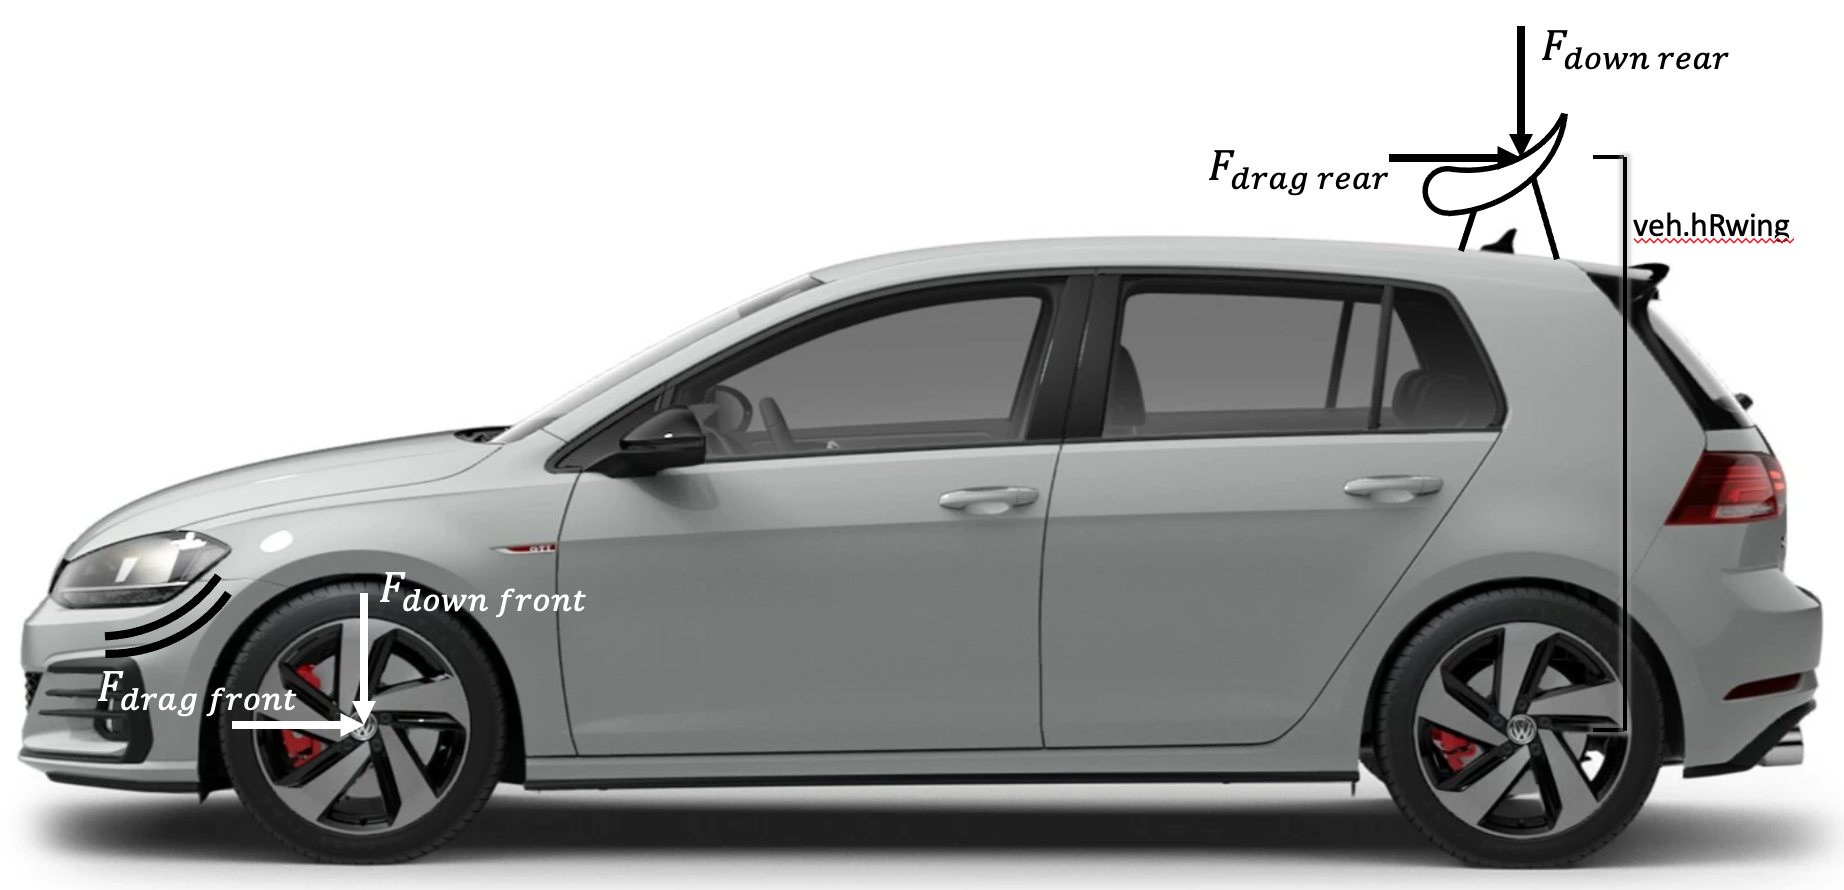
\includegraphics[width=400pt]{Template/Problem4/fbd_gti.png}
\url{https://www.vw.com/en/models/golf-gti.html}
\end{center}

\textit{Note: The drag on the rear wing will have an impact on the downforce on the front axle. Be sure to account for this.}

Restore Niki's brake distribution to the original 64/36.  Now, simulate the same curve as in the previous problem.   How does the distance covered compare to Question 3C?  How does the maximum lateral error compare to 3C? Plot the front and rear tire forces. Provide the plots and describe what is happening.  Does it make sense to add an aero kit to Niki?

\vspace*{0.5cm}

\expect{Run the simulation and answer the questions about the vehicle's behavior.  Was it a good idea to upgrade Niki? Include the tire force plots.}

\iftoggle{condensed}{
    \vspace*{0.5cm}
}{
    \subsubsection*{Solution:}
}

\iftoggle{solution}{
    %---------------------------------------------------------------------------------
% QUESTION 4.A
%---------------------------------------------------------------------------------
\secMOGS{Adding Aerodynamics}

Modify \verb!aero_effects.m! to implement the added downforce and drag from the wing.  We can assume that the front wing aero forces act at the center of the front wheel and that the rear wing aero forces act at a distance \verb!veh.hRwing! directly above the rear wheel. We can also assume that the front wing acts equally on the left and right front wheels and that the rear wing acts equally on the left and right rear wheels. Here is a free body diagram of the GTI with the forces we added with the two wings.    

\begin{center}
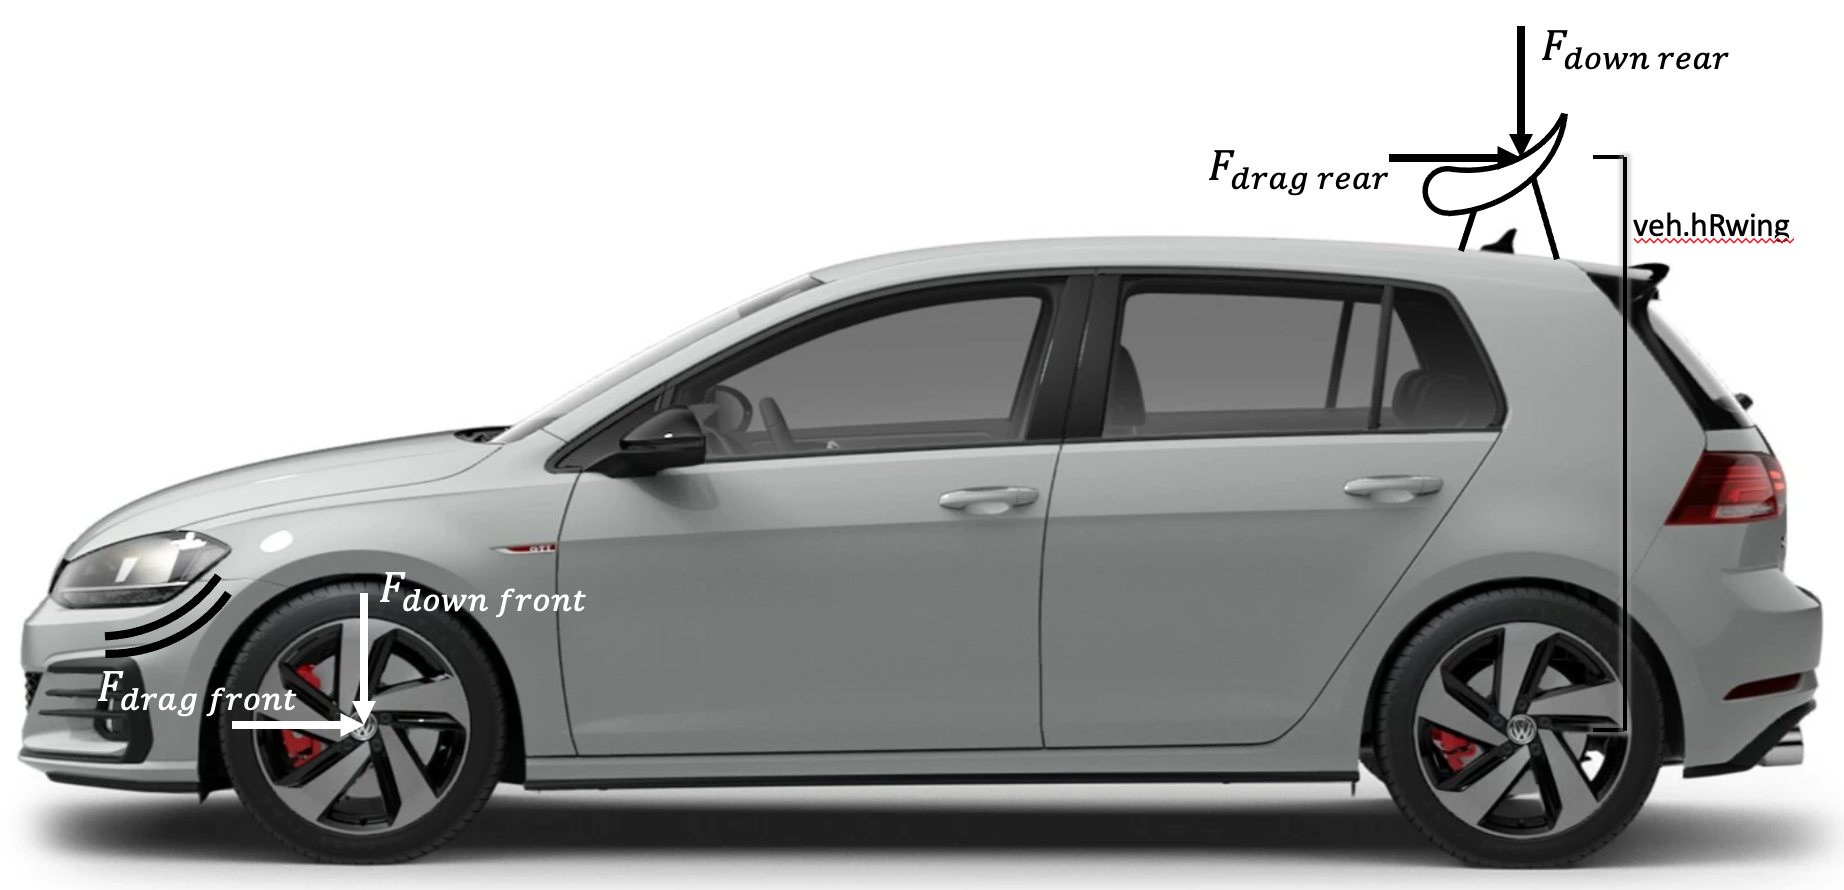
\includegraphics[width=400pt]{Template/Problem4/fbd_gti.png}
\url{https://www.vw.com/en/models/golf-gti.html}
\end{center}

\textit{Note: The drag on the rear wing will have an impact on the downforce on the front axle. Be sure to account for this.}

Restore Niki's brake distribution to the original 64/36.  Now, simulate the same curve as in the previous problem.   How does the distance covered compare to Question 3C?  How does the maximum lateral error compare to 3C? Plot the front and rear tire forces. Provide the plots and describe what is happening.  Does it make sense to add an aero kit to Niki?

\vspace*{0.5cm}

\expect{Run the simulation and answer the questions about the vehicle's behavior.  Was it a good idea to upgrade Niki? Include the tire force plots.}

\iftoggle{condensed}{
    \vspace*{0.5cm}
}{
    \subsubsection*{Solution:}
}

\iftoggle{solution}{
    %---------------------------------------------------------------------------------
% QUESTION 4.A
%---------------------------------------------------------------------------------
\secMOGS{Adding Aerodynamics}

Modify \verb!aero_effects.m! to implement the added downforce and drag from the wing.  We can assume that the front wing aero forces act at the center of the front wheel and that the rear wing aero forces act at a distance \verb!veh.hRwing! directly above the rear wheel. We can also assume that the front wing acts equally on the left and right front wheels and that the rear wing acts equally on the left and right rear wheels. Here is a free body diagram of the GTI with the forces we added with the two wings.    

\begin{center}
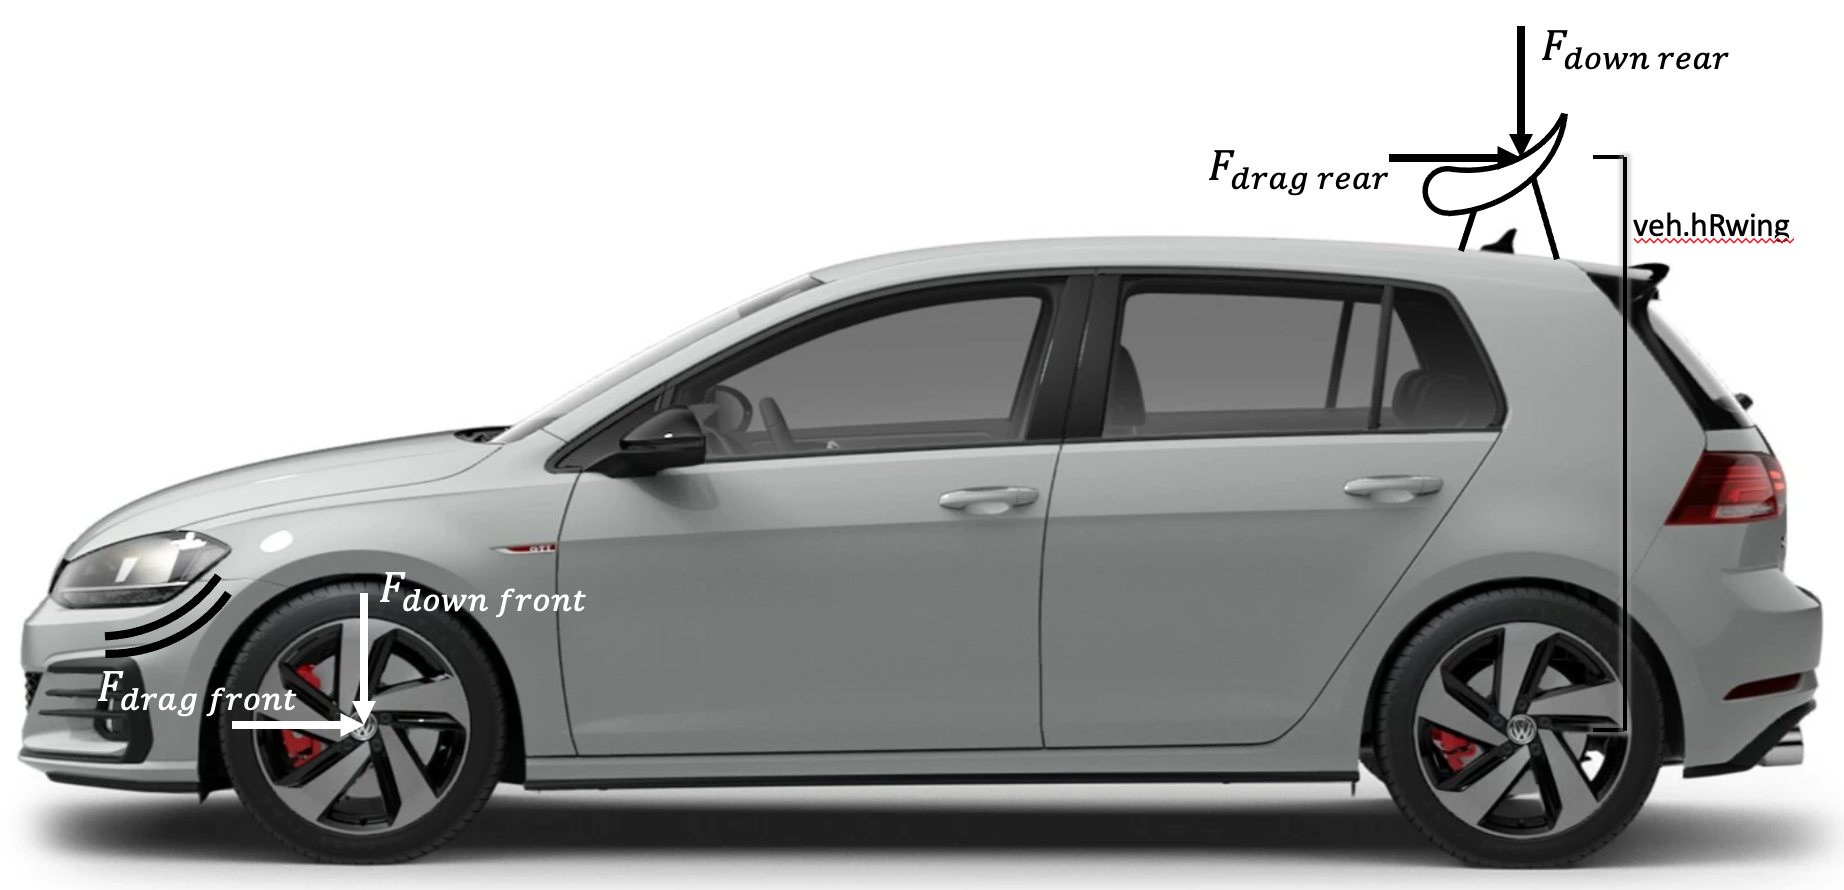
\includegraphics[width=400pt]{Template/Problem4/fbd_gti.png}
\url{https://www.vw.com/en/models/golf-gti.html}
\end{center}

\textit{Note: The drag on the rear wing will have an impact on the downforce on the front axle. Be sure to account for this.}

Restore Niki's brake distribution to the original 64/36.  Now, simulate the same curve as in the previous problem.   How does the distance covered compare to Question 3C?  How does the maximum lateral error compare to 3C? Plot the front and rear tire forces. Provide the plots and describe what is happening.  Does it make sense to add an aero kit to Niki?

\vspace*{0.5cm}

\expect{Run the simulation and answer the questions about the vehicle's behavior.  Was it a good idea to upgrade Niki? Include the tire force plots.}

\iftoggle{condensed}{
    \vspace*{0.5cm}
}{
    \subsubsection*{Solution:}
}

\iftoggle{solution}{
    \input{Solutions/Problem4/problem4a.tex}
    \newpage
}

\iftoggle{template}{
    \begin{solutionorbox}[3.5in]
    \end{solutionorbox}
    \newpage
}

\iftoggle{student}{
%---------------------------------------------------------------------------------
% STUDENT: BEGIN WORK
%---------------------------------------------------------------------------------


% Please box final answer

%---------------------------------------------------------------------------------
% STUDENT: END WORK
%---------------------------------------------------------------------------------
    \newpage
}












    \newpage
}

\iftoggle{template}{
    \begin{solutionorbox}[3.5in]
    \end{solutionorbox}
    \newpage
}

\iftoggle{student}{
%---------------------------------------------------------------------------------
% STUDENT: BEGIN WORK
%---------------------------------------------------------------------------------


% Please box final answer

%---------------------------------------------------------------------------------
% STUDENT: END WORK
%---------------------------------------------------------------------------------
    \newpage
}












    \newpage
}

\iftoggle{template}{
    \begin{solutionorbox}[3.5in]
    \end{solutionorbox}
    \newpage
}

\iftoggle{student}{
%---------------------------------------------------------------------------------
% STUDENT: BEGIN WORK
%---------------------------------------------------------------------------------


% Please box final answer

%---------------------------------------------------------------------------------
% STUDENT: END WORK
%---------------------------------------------------------------------------------
    \newpage
}













\newpage

%---------------------------------------------------------------------------------
% REMARKS
%---------------------------------------------------------------------------------
\iftoggle{solution}{
    \input{Solutions/remarks.tex}
    \newpage
}

%---------------------------------------------------------------------------------
% APPENDICES
%---------------------------------------------------------------------------------
\appendix
\secApp{Vehicle Parameters}

\renewcommand{\arraystretch}{2}
\begin{table}[h!]
    \centering
    \begin{tabular}{| l | r | c | l |}
        \hline
        \bld{Variable Name} & \bld{Value} & \bld{Units} & \bld{Description} \\[5pt]
        \hline\hline
        \verb$veh.m$  & 1926.2  & \si{\kg}     & Mass (Includes 4 passengers)               \\ \hline
        \verb$veh.Iz$ & 2763.49 & \si{\kg.\m^2} & Yaw Moment of Inertia                      \\ \hline
        \verb$veh.a$  & 1.264   & \si{\m}      & Distance from Center of Mass to Front Axle \\ \hline
        \verb$veh.b$  & 1.367   & \si{\m}      & Distance from Center of Mass to Rear Axle  \\ \hline
        \verb$veh.L$  & 2.631   & \si{\m}      & Wheelbase                                  \\ \hline
        \verb$veh.Wf$ & 9817.9  & \si{\N}      & Static front axle weight                   \\ \hline
        \verb$veh.Wr$ & 9078.1  & \si{\N}      & Static rear axle weight                    \\ \hline
    \end{tabular}
    \caption{Vehicle Parameters and Values}
    \label{Table:VehParams}
\end{table}
\renewcommand{\arraystretch}{1}

\newpage

\secApp{Tire Parameters}

\subsection*{Linear Tire Model}

\renewcommand{\arraystretch}{2}
\begin{table}[h!]
    \centering
    \begin{tabular}{| l | c | c | l |}
    \hline
    \bld{Variable Name} & \bld{Value} & \bld{Units} & \bld{Description} \\[5pt]
    \hline\hline
    \verb$f_tire.ca_lin$  & 80,000 & \si{\N/\radian} & Front Cornering Stiffness \\ \hline
    \hline
    \verb$r_tire.ca_lin$ & 120,000 & \si{\N/\radian} & Rear Cornering Stiffness  \\ \hline
    \end{tabular}
    \caption{Linear Tire Model Parameters}
    \label{Table:LinTire}
\end{table}

\vspace*{0.5cm}

\subsection*{Fiala Tire Model}

\begin{table}[h!]
    \centering
    \begin{tabular}{| l | c | c | l |}
    \hline
    \bld{Variable Name} & \bld{Value} & \bld{Units} & \bld{Description} \\[5pt]
    \hline\hline
    \verb$f_tire.cy$    & 110,000 & \si{\N/\radian} & Front Cornering Stiffness             \\\hline
    \verb$f_tire.mu$    &    0.90 & Unitless        & Front Peak Coefficient of Friction    \\\hline
    \verb$f_tire.mu_s$  &    0.90 & Unitless        & Front Sliding Coefficient of Friction \\\hline
    \hline
    \verb$r_tire.cy$    & 180,000 & \si{\N/\radian} & Rear Cornering Stiffness              \\\hline
    \verb$r_tire.mu$    &    0.94 & Unitless        & Rear Peak Coefficient of Friction     \\\hline
    \verb$r_tire.mu_s$  &    0.94 & Unitless        & Rear Sliding Coefficient of Friction  \\\hline
    \end{tabular}
    \caption{Fiala Tire Model Parameters}
    \label{Table:FialaTire}
\end{table}
\renewcommand{\arraystretch}{1}
\newpage

\secApp{MATLAB}


\subsection*{MATLAB Background}

MATLAB is widely used in the automotive industry and in engineering more generally.  As a result of its broad application, MATHWORKS has developed various toolboxes for industry-specific needs.  Given this, it's often not necessary to download all toolboxes that MATHWORKS offers and companies will usually purchase only the toolboxes that are needed by their engineers.  

\subsection*{MATLAB Installation}
To install MATLAB and any associated toolboxes, go to the MATHWORKS website (\url{www.mathworks.com}) and create an account using your Stanford email. This will give you access to the complete version of MATLAB. Follow the instructions on the MATHWORKS website to download the software.


\subsection*{MATLAB Version}
Mathworks tries to give both backward and forward compatibility to MATLAB.  This is not always true and is especially tricky with certain toolboxes.  Downloading the latest version of MATLAB (2021a) should work for everything we're doing in this class.  If you already have an older version of MATLAB installed on your computer, don't worry about upgrading to the latest version.  Should any compatibility issues arise, the teaching team will handle them with you on a case-by-case basis.

\subsection*{MATLAB Toolboxes}
We require downloading these toolboxes in order to use the framework we have developed for the project:
\\MATLAB 2021a
\\Control System Toolbox
\\DSP System Toolbox

Simulink and Stateflow will not be used in this class, but they are widely used in research and industry.  You may find it helpful to download these now for future use.  You can always return later to download additional toolboxes.



\end{document}
